\begin{psfrags}%
\psfragscanon

% text strings:
\psfrag{t01}[bc]{$n_1 = 1,N_p$}
\psfrag{t02}[bc]{$\theta_1=\frac{2\pi}{2m}(n_1-1)$}
\psfrag{t03}[bc]{$\theta_2=\frac{2\pi}{2m}n_1$}
\psfrag{t04}[bc]{$k=f(n_1,m)$}
\psfrag{t05}[bc]{$n_2 = 1,Q_s$}
\psfrag{t06}[bc]{$\theta_e = p\alpha_{n_2}$}
\psfrag{t07}[bc]{$\theta_1 \leq \theta_e < \theta_2$}
\psfrag{t08}[bc]{$i=f(k)$ and $h=-1^{(k-1)}$}
\psfrag{t09}[bc]{$\mathbf{M}_{1,ij}=h \quad j=n_2$}
\psfrag{t10}[bc]{$\mathbf{M}_{2,ij}=-h \quad j=f(n_2,y_d)$}
\psfrag{t11}[bc]{$n_2=Q_s$?}
\psfrag{t12}[bc]{$n_1=N_p$?}
\psfrag{t13}[bc]{End}
\psfrag{t14}[bc]{Start}
\psfrag{t15}[bc]{$\mathbf{M}_{ij} \in \left\{-1,1\right\}$}

\psfrag{t16}[bc]{$\mod(n_2,2)=0$}
\psfrag{t17}[br]{Phase belt constraint}
\psfrag{t18}[br]{Inner loop (slots)}
\psfrag{t19}[br]{Outer loop (phase belts)}

\psfrag{t20}[bc]{$\tau_s=\frac{2\pi}{Q_s}$}
\psfrag{t21}[bl]{\eqref{eqn:phase_belt_number}}

\psfrag{t22}[bl]{\eqref{eqn:slot_alpha}}
\psfrag{t23}[bl]{\eqref{eqn:Np}}

\psfrag{t24}[bc]{$\mbox{mod}\bigl(\frac{Q_s}{t},m\bigr)=0$}
\psfrag{t25}[bc]{End}
\psfrag{t26}[bl]{Table \ref{tab:feasibility}}
\psfrag{t27}[bc]{$\xi_{\nu} = \frac{m}{2Q_c}(                              
                  \mathbf{M}_1\mathbf{v}_{\nu}+\mathbf{M}_2\mathbf{v}_{\nu})$}
\psfrag{t28}[bl]{\eqref{eqn:winding_factor}}
\psfrag{t29}[br]{Section \ref{sec:m_assignment}}
\psfrag{t30}[bl]{\eqref{eqn:phase_belt_constraint}}
\psfrag{t31}[bl]{Symmetry test:}
\psfrag{t32}[bl]{\eqref{eqn:matrix_element}}
\psfrag{t33}[bc]{y}
\psfrag{t34}[bc]{n}

% Figure:
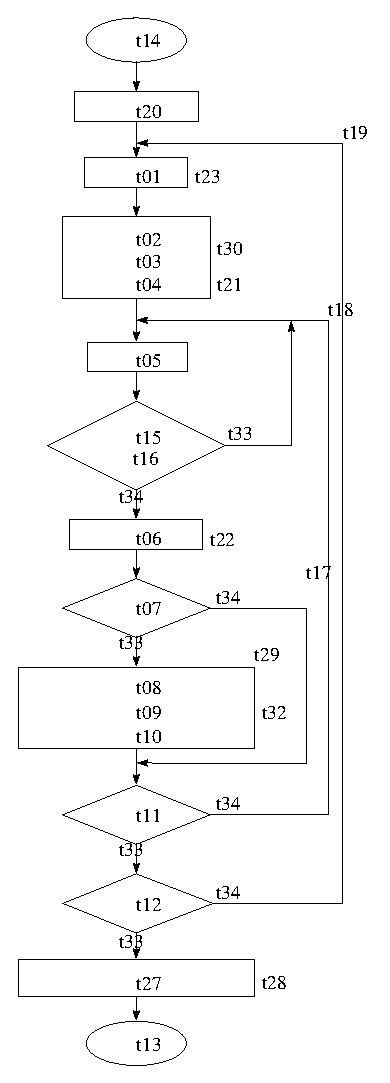
\includegraphics[width=0.47\textwidth]{figs/f_flowchart.eps}
\end{psfrags}%